\documentclass[12pt]{article}
\usepackage{graphicx}
\usepackage[latin1]{inputenc}
\usepackage{amsmath}
\usepackage{calc}
\usepackage{amssymb}

\textwidth = 15.5 true cm
\topmargin=-1.0truecm
\evensidemargin=0pt
\oddsidemargin=0pt
\parindent=0pt
\frenchspacing
\pagestyle{empty}

\newcommand{\HRule}{\rule{\linewidth}{0.075mm}}

\newlength{\depthofsumsign}
\setlength{\depthofsumsign}{\depthof{$\sum$}}
\newcommand{\nsum}[1][1.4]{\mathop{\raisebox{-#1\depthofsumsign+1\depthofsumsign}{\scalebox{#1}{$\displaystyle\sum$}}}}

\begin{document}

\parbox[t]{8cm}{\textsf{Course 02249 Computationally Hard Problems\\
Fall 2013, DTU Compute }}
\hfill
\parbox[t]{1cm}{\mbox{}\\
\raisebox{0.0cm}[1cm][1cm]{
\includegraphics[origin=lb]{dtu_logo.pdf}}}

{\Large  Solution to assignment \textsc{Project}\\[4mm]
Students' names: Andreas Hallberg Kjeldsen and Morten Chabert Eskesen\\[4mm]
Study nr. s092638 and s133304\\[4mm]
Date. 04\textbf{.}11\textbf{.}2013 }


\vspace{7cm}

\begin{center}
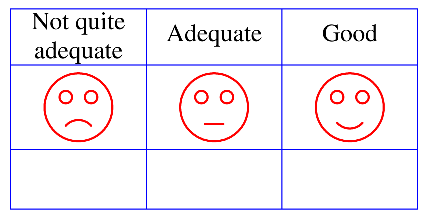
\includegraphics[scale=1.0]{Evurd.pdf}
\end{center}

\newpage

\HRule\\
\textbf{Problem:} \textsc{[MirrorFriendlyMinimumSpanningTree (MFMST)]}\\
\textbf{Input:} An undirected, connected weighted graph $G = (V,E,w)$, where $V = \{1,\dots,n\}$, $E = \{e_1,\dots,e_m\}$ and $w : E \rightarrow \mathbb{N}_0$, and a number $B \in \mathbb{N}$.\\
\textbf{Output:} YES if there is a spanning tree $T \subseteq E$ for $G$ such that
$$max \left\{\nsum\limits_{e_i \in T} w(e_i), \nsum\limits_{e_i \in T} w(e_{m+1-i})\right\} \leq B$$
and NO otherwise.\\
\HRule

\subsection*{a) Description of the problem in colloquial terms}
A minimum spanning tree is a subgraph within a undirected, connected weighted graph that is a tree and connects all the vertices together with a weight less or equal to the weight of every other spanning tree. The main difference between a minimum spanning tree and a mirror friendly minimum spanning tree is the inequality described above. In a mirror friendly minimum spanning tree the inequality must be satisfied. It should be possible to mirror the spanning tree in such a way that the maximum of the spanning tree and the mirrored spanning tree is less than or equal to a fixed value, $B$. This also means that the mirror friendly minimum spanning tree may not be equal to the minimum spanning tree in the graph, i.e. it may have a larger weight than the minimum spanning tree.

\subsubsection*{Solve an example problem}
\textbf{Input:} $V = \{1,2,3\}$, $E = \{e_1 = \{1,2\},e_2 = \{2,3\},e_3 = \{1,3\}\}$, $w(e_i) = i$ for $i \in \{1,2,3\}$ and $B = 4$.
\begin{center}
\begin{tabular}{ c c }
Spanning Tree & Mirrored Spanning Tree\\
$e_1 + e_2 = 3$ & $e_{3+1-1} + e_{3+1-2} = 5$\\
$e_3 + e_1 = 4$ & $e_{3+1-3} + e_{3+1-1} = 4$\\
\end{tabular}
\end{center}
$$max \left\{e_3 + e_1, e_{3+1-3} + e_{3+1-1}\right\} \leq 4$$
$$max \left\{4, 4\right\} \leq 4$$
Output would be a spanning tree consisting of the edges: $e_3$ and $e_1$.
\subsection*{b) Show that MFMST is in $NP$}
\subsubsection*{1. Design a deterministic algorithm $A$ which takes as input a problem instance $X$ and random sequence $R$}

\textbf{1a. Specify what the random sequence $R$ consists of}\\

\textbf{1b. Specify how $A$ interprets $R$ as a guess}\\

\textbf{1c. Specify how $A$ verifies the guess}\\

\subsubsection*{2. Show that the two conditions are met}

\textbf{If the answer to $X$ is YES, then there is a string $R^*$ with positive probability such that $A(X, R^*) = YES$}\\

\textbf{If the answer to $X$ is NO, then $A(X, R) = NO$ for all $R$}\\

\subsubsection*{3. Show that $A$ is $p$-bounded for some polynomial $p$}

\subsection*{c) Show that MFMST is $NP$-complete}
\subsubsection*{Suitable problem $P_c$ known to be $NP$-complete}

Prove $P_c \leq_p$ \textsc{MirrorFriendlyMinimumSpanningTree}.

\textbf{Outline of the transformation}\\

\textbf{Answer to $X$ is YES then answer to $T(X)$ is YES}\\

\textbf{Answer to $T(X)$ is YES then answer to $X$ is YES}\\

\textbf{Time Analysis}

\subsection*{d) Find an algorithm which solves the optimizing version of the problem}


\subsection*{e) Prove the worst-case running time of the algorithm}


\subsection*{f) Implement the algorithm developed in d)}


\end{document}
